\documentclass[11pt, spanish]{report}
\usepackage[spanish]{babel}
\usepackage[utf8]{inputenc}
\usepackage{geometry}
\usepackage{graphicx}
\usepackage{subfig}
\usepackage{caption}
\usepackage{subcaption}
 \geometry{
 a4paper,
 total={170mm,257mm},
 left=20mm,
 top=20mm,
 }
\usepackage{graphicx}
\graphicspath{ {images/} }
\usepackage[utf8]{inputenc}
\decimalpoint
\title{Actividad 7: Visualización de datos con la biblioteca Seaborn}
\author{César Andrés Pérez Robinson }
\date{Marzo 2019}

\begin{document}

\maketitle

\section{Introducción}
En esta actividad se analizan datos de una estación de meteorología ubicada en un campo de nogal. Se descargan datos del año 2009 y parte del 2010. \\
Se aprende a eliminar múltiples columnas sin nombre y con datos vacíos de nuestra base de datos, de manera en que solamente se trabaja con los datos útiles. \\
Después se aprende a realizar correlaciones o dependencia entre variables y después se utiliza Matplotlib y Seaborn para realizar un mapa de correlaciones y se compara el uso de Seaborn y Matplotlib. \\
Por último, se realizan gráficas de dispersión en aquellas variables conde la correlación sea mayor a 0.6 entre ellas.
\section{Código y desarrollo}
De manera inicial, se descargan las librerías con las cuales se trabajará:
\begin{verbatim}
from string import ascii_letters
import numpy as np
import pandas as pd
import seaborn as sns
import matplotlib.pyplot as plt
import math
\end{verbatim}
Y se descarga el archivo de datos y se observa el tipo de datos:
\begin{verbatim}
[IN]
df = pd.read_csv('meteonogal.csv', sep=',', engine='python')
df.dtypes

[OUT]
DATE            object
TIME            object
Unnamed: 2     float64
Unnamed: 3     float64
u_Avg           object
v_Avg           object
w_Avg           object
t_Avg           object
kh20_Avg        object
net_rad_Avg     object
shf1_Avg        object
shf2_Avg        object
vv_Avg          object
airT_Avg        object
rh_Avg         float64
e_sat_Avg       object
e_Avg           object
h2o_hmp_Avg     object
Unnamed: 18    float64
Unnamed: 19     object
Unnamed: 20     object
Unnamed: 21    float64
Unnamed: 22     object
Unnamed: 23     object
Unnamed: 24     object
Unnamed: 25     object
Unnamed: 26     object
Unnamed: 27     object
Unnamed: 28     object
Unnamed: 29     object
Unnamed: 30     object
Unnamed: 31     object
Unnamed: 32     object
Unnamed: 33     object
Unnamed: 34     object
Unnamed: 35     object
dtype: object
\end{verbatim}
Se observa que se encuentra un gran número de columnas sin nombre y sin datos, por lo que se eliminan de la base de datos: 
\begin{verbatim}
[IN]
# para eliminar columnas sin información, se buscó la manera
# de eliminar aquellas que no estén nombradas 'unnamed'
df = df.drop(df.columns[df.columns.str.contains('unnamed:',case = False)],axis = 1)
df.head()

[OUT]
DATE            object
TIME            object
u_Avg           object
v_Avg           object
w_Avg           object
t_Avg           object
kh20_Avg        object
net_rad_Avg     object
shf1_Avg        object
shf2_Avg        object
vv_Avg          object
airT_Avg        object
rh_Avg         float64
e_sat_Avg       object
e_Avg           object
h2o_hmp_Avg     object
dtype: object
\end{verbatim}
Ya que el primer renglón de la base de datos solamente muestra las unidades con las que se mide cada variable, también se elimina.
\begin{verbatim}
df = df.drop([0], axis=0)
\end{verbatim}
Se hacen convierten las variables a "float".
\begin{verbatim}
[IN
]df[df.columns[2:16]] = df[df.columns[2:16]].astype(float)
df.dtypes

[OUT]
DATE            object
TIME            object
u_Avg          float64
v_Avg          float64
w_Avg          float64
t_Avg          float64
kh20_Avg       float64
net_rad_Avg    float64
shf1_Avg       float64
shf2_Avg       float64
vv_Avg         float64
airT_Avg       float64
rh_Avg         float64
e_sat_Avg      float64
e_Avg          float64
h2o_hmp_Avg    float64
dtype: object
\end{verbatim}
Se realiza una matríz de correlaciones:
\begin{verbatim}
corr = df.corr()
corr
\end{verbatim}
Se utiliza Seaborn para generar un mapa de correlaciones, cuyo resultado se muestra en la Figura 1.
\begin{verbatim}
#Utilizando Seaborn

# Generate a mask for the upper triangle
mask = np.zeros_like(corr, dtype=np.bool)
mask[np.triu_indices_from(mask)] = True

# Set up the matplotlib figure
f, ax = plt.subplots(figsize=(11, 9))

# Generate a custom diverging colormap
cmap = sns.diverging_palette(220, 10, as_cmap=True)

# Draw the heatmap with the mask and correct aspect ratio
sns.heatmap(corr, mask=mask, cmap=cmap, vmax=.3, center=0,
            square=True, linewidths=.5, cbar_kws={"shrink": .5})
\end{verbatim}
\begin{figure}[ht]
\caption{Mapa de correlaciones Seaborn}
\centering
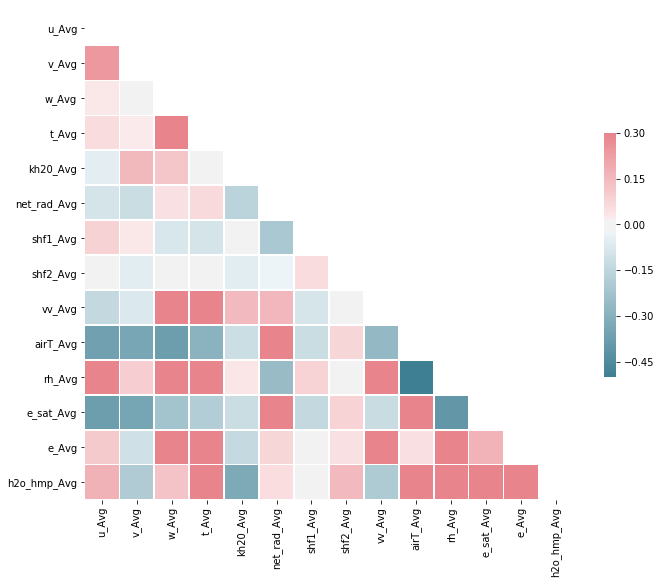
\includegraphics[width=0.65\textwidth]{Seaborn.png}
\end{figure}
Después se genera el mismo mapa de correlaciones utilizando Matplotlib y se muestra en la Figura 2.
\begin{verbatim}
#Utilizando Matplotlib.
fig, matriz = plt.subplots()                    

#Establecemos el tamaño de los ejes.
matriz.set_xticks(np.arange(len(corr)))      
matriz.set_yticks(np.arange(len(corr)))

#Mostrando los nombre de cada variable
matriz.set_xticklabels(corr)                 
matriz.set_yticklabels(corr.columns[::-1])

#rotando las etiquetas
plt.setp(matriz.get_xticklabels(), rotation=80, ha="right",rotation_mode="anchor")

#Graficamos las correlaciones
plt.imshow(corr,cmap='viridis', interpolation='nearest')


matriz.set_title("Matplotlib")   
plt.show()
\end{verbatim}
\begin{figure}[ht]
\caption{Mapa de correlaciones Matplotlib}
\centering
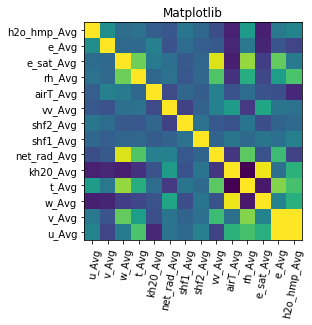
\includegraphics[width=0.65\textwidth]{matplotlib.png}
\end{figure}
Se realizan gráficas de dispersiones con aquellas variables cuyas correlaciones fueron mayores a 0.6.
\begin{verbatim}
w_Avg y t_Avg con corr = 0.667294 en Figura 3
w_Avg y vv_Avg con corr = 0.923685 en Figura 4
w_Avg y rh_Avg con corr = 0.760058 en Figura 5
w_Avg y e_Avg con corr = 0.641772 en Figura 6
vv_Avg y rh_Avg con corr = 0.624201 en Figura 7
airT_Avg y e_sat_Avg con corr = 0.963527 en Figura 8
rh_Avg y e_Avg con corr = 0.722503 en Figura 9
e_Avg y h2o_hmp_Avg con corr = 0.999154 en Figura 10
\end{verbatim}
\begin{figure}
\centering
\begin{minipage}{.5\textwidth}
  \centering
  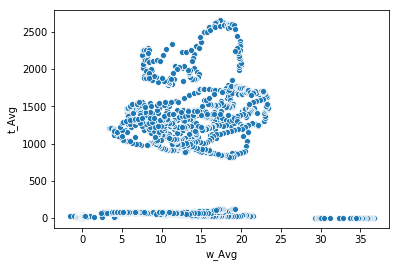
\includegraphics[width=\linewidth]{1.png}
  \captionof{figure}{w\_Avg y t\_Avg. Corr = 0.667}
  \label{fig:test1}
\end{minipage}%
\begin{minipage}{.5\textwidth}
  \centering
  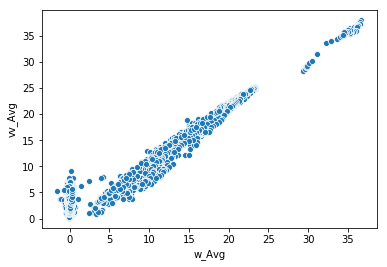
\includegraphics[width=\linewidth]{2.png}
  \captionof{figure}{w\_Avg y vv\_Avg. Corr = 0.923}
  \label{fig:test2}
\end{minipage}
\end{figure}
\begin{figure}
\centering
\begin{minipage}{.5\textwidth}
  \centering
  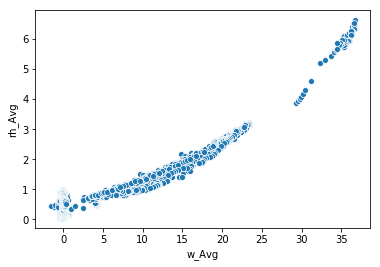
\includegraphics[width=\linewidth]{3.png}
  \captionof{figure}{w\_Avg y rh\_Avg. Corr = 0.760}
  \label{fig:test1}
\end{minipage}%
\begin{minipage}{.5\textwidth}
  \centering
  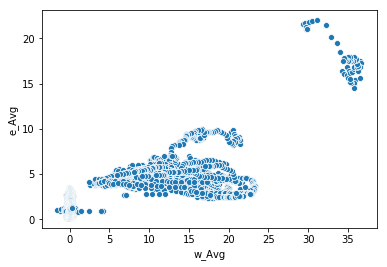
\includegraphics[width=\linewidth]{4.png}
  \captionof{figure}{w\_Avg y e\_Avg. Corr = 0.641}
  \label{fig:test2}
\end{minipage}
\end{figure}
\begin{figure}
\centering
\begin{minipage}{.5\textwidth}
  \centering
  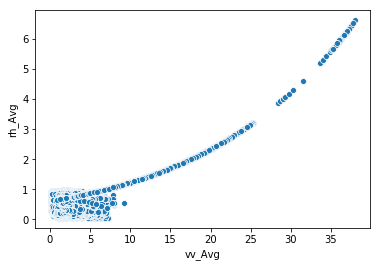
\includegraphics[width=\linewidth]{5.png}
  \captionof{figure}{vv\_Avg y rh\_Avg. Corr = 0.624}
  \label{fig:test1}
\end{minipage}%
\begin{minipage}{.5\textwidth}
  \centering
  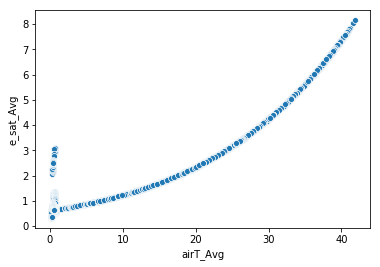
\includegraphics[width=\linewidth]{6.png}
  \captionof{figure}{airT\_Avg y e\_Avg. Corr = 0.963}
  \label{fig:test2}
\end{minipage}
\end{figure}
\begin{figure}
\centering
\begin{minipage}{.5\textwidth}
  \centering
  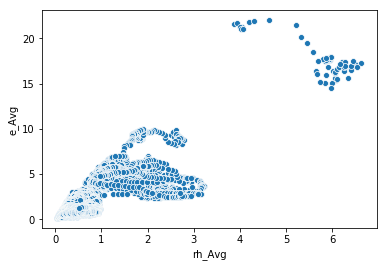
\includegraphics[width=\linewidth]{7.png}
  \captionof{figure}{rh\_Avg y e\_Avg. Corr = 0.722}
  \label{fig:test1}
\end{minipage}%
\begin{minipage}{.5\textwidth}
  \centering
  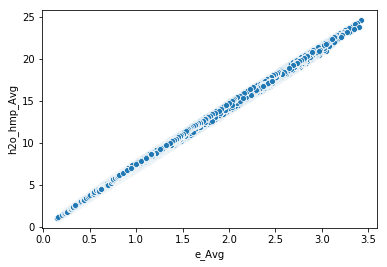
\includegraphics[width=\linewidth]{8.png}
  \captionof{figure}{e\_Avg y h2o\_hmp\_Avg. Corr = 0.999}
  \label{fig:test2}
\end{minipage}
\end{figure}
\section{Comentarios finales}
La utilización de Seaborn representa una manera más facil e ilustrativa de representar los datos, muestra una variedad de imágenes coloridas y fáciles de generar así como interpretar.
\end{document}
